\PassOptionsToPackage{unicode=true}{hyperref} % options for packages loaded elsewhere
\PassOptionsToPackage{hyphens}{url}
%
\documentclass[]{article}
\usepackage{lmodern}
\usepackage{amssymb,amsmath}
\usepackage{ifxetex,ifluatex}
\usepackage{fixltx2e} % provides \textsubscript
\ifnum 0\ifxetex 1\fi\ifluatex 1\fi=0 % if pdftex
  \usepackage[T1]{fontenc}
  \usepackage[utf8]{inputenc}
  \usepackage{textcomp} % provides euro and other symbols
\else % if luatex or xelatex
  \usepackage{unicode-math}
  \defaultfontfeatures{Ligatures=TeX,Scale=MatchLowercase}
\fi
% use upquote if available, for straight quotes in verbatim environments
\IfFileExists{upquote.sty}{\usepackage{upquote}}{}
% use microtype if available
\IfFileExists{microtype.sty}{%
\usepackage[]{microtype}
\UseMicrotypeSet[protrusion]{basicmath} % disable protrusion for tt fonts
}{}
\IfFileExists{parskip.sty}{%
\usepackage{parskip}
}{% else
\setlength{\parindent}{0pt}
\setlength{\parskip}{6pt plus 2pt minus 1pt}
}
\usepackage{hyperref}
\hypersetup{
            pdftitle={Using Both R and Python to Manipulate Data},
            pdfauthor={Kathleen Strybos},
            pdfborder={0 0 0},
            breaklinks=true}
\urlstyle{same}  % don't use monospace font for urls
\usepackage[margin=1in]{geometry}
\usepackage{color}
\usepackage{fancyvrb}
\newcommand{\VerbBar}{|}
\newcommand{\VERB}{\Verb[commandchars=\\\{\}]}
\DefineVerbatimEnvironment{Highlighting}{Verbatim}{commandchars=\\\{\}}
% Add ',fontsize=\small' for more characters per line
\usepackage{framed}
\definecolor{shadecolor}{RGB}{248,248,248}
\newenvironment{Shaded}{\begin{snugshade}}{\end{snugshade}}
\newcommand{\AlertTok}[1]{\textcolor[rgb]{0.94,0.16,0.16}{#1}}
\newcommand{\AnnotationTok}[1]{\textcolor[rgb]{0.56,0.35,0.01}{\textbf{\textit{#1}}}}
\newcommand{\AttributeTok}[1]{\textcolor[rgb]{0.77,0.63,0.00}{#1}}
\newcommand{\BaseNTok}[1]{\textcolor[rgb]{0.00,0.00,0.81}{#1}}
\newcommand{\BuiltInTok}[1]{#1}
\newcommand{\CharTok}[1]{\textcolor[rgb]{0.31,0.60,0.02}{#1}}
\newcommand{\CommentTok}[1]{\textcolor[rgb]{0.56,0.35,0.01}{\textit{#1}}}
\newcommand{\CommentVarTok}[1]{\textcolor[rgb]{0.56,0.35,0.01}{\textbf{\textit{#1}}}}
\newcommand{\ConstantTok}[1]{\textcolor[rgb]{0.00,0.00,0.00}{#1}}
\newcommand{\ControlFlowTok}[1]{\textcolor[rgb]{0.13,0.29,0.53}{\textbf{#1}}}
\newcommand{\DataTypeTok}[1]{\textcolor[rgb]{0.13,0.29,0.53}{#1}}
\newcommand{\DecValTok}[1]{\textcolor[rgb]{0.00,0.00,0.81}{#1}}
\newcommand{\DocumentationTok}[1]{\textcolor[rgb]{0.56,0.35,0.01}{\textbf{\textit{#1}}}}
\newcommand{\ErrorTok}[1]{\textcolor[rgb]{0.64,0.00,0.00}{\textbf{#1}}}
\newcommand{\ExtensionTok}[1]{#1}
\newcommand{\FloatTok}[1]{\textcolor[rgb]{0.00,0.00,0.81}{#1}}
\newcommand{\FunctionTok}[1]{\textcolor[rgb]{0.00,0.00,0.00}{#1}}
\newcommand{\ImportTok}[1]{#1}
\newcommand{\InformationTok}[1]{\textcolor[rgb]{0.56,0.35,0.01}{\textbf{\textit{#1}}}}
\newcommand{\KeywordTok}[1]{\textcolor[rgb]{0.13,0.29,0.53}{\textbf{#1}}}
\newcommand{\NormalTok}[1]{#1}
\newcommand{\OperatorTok}[1]{\textcolor[rgb]{0.81,0.36,0.00}{\textbf{#1}}}
\newcommand{\OtherTok}[1]{\textcolor[rgb]{0.56,0.35,0.01}{#1}}
\newcommand{\PreprocessorTok}[1]{\textcolor[rgb]{0.56,0.35,0.01}{\textit{#1}}}
\newcommand{\RegionMarkerTok}[1]{#1}
\newcommand{\SpecialCharTok}[1]{\textcolor[rgb]{0.00,0.00,0.00}{#1}}
\newcommand{\SpecialStringTok}[1]{\textcolor[rgb]{0.31,0.60,0.02}{#1}}
\newcommand{\StringTok}[1]{\textcolor[rgb]{0.31,0.60,0.02}{#1}}
\newcommand{\VariableTok}[1]{\textcolor[rgb]{0.00,0.00,0.00}{#1}}
\newcommand{\VerbatimStringTok}[1]{\textcolor[rgb]{0.31,0.60,0.02}{#1}}
\newcommand{\WarningTok}[1]{\textcolor[rgb]{0.56,0.35,0.01}{\textbf{\textit{#1}}}}
\usepackage{graphicx,grffile}
\makeatletter
\def\maxwidth{\ifdim\Gin@nat@width>\linewidth\linewidth\else\Gin@nat@width\fi}
\def\maxheight{\ifdim\Gin@nat@height>\textheight\textheight\else\Gin@nat@height\fi}
\makeatother
% Scale images if necessary, so that they will not overflow the page
% margins by default, and it is still possible to overwrite the defaults
% using explicit options in \includegraphics[width, height, ...]{}
\setkeys{Gin}{width=\maxwidth,height=\maxheight,keepaspectratio}
\setlength{\emergencystretch}{3em}  % prevent overfull lines
\providecommand{\tightlist}{%
  \setlength{\itemsep}{0pt}\setlength{\parskip}{0pt}}
\setcounter{secnumdepth}{0}
% Redefines (sub)paragraphs to behave more like sections
\ifx\paragraph\undefined\else
\let\oldparagraph\paragraph
\renewcommand{\paragraph}[1]{\oldparagraph{#1}\mbox{}}
\fi
\ifx\subparagraph\undefined\else
\let\oldsubparagraph\subparagraph
\renewcommand{\subparagraph}[1]{\oldsubparagraph{#1}\mbox{}}
\fi

% set default figure placement to htbp
\makeatletter
\def\fps@figure{htbp}
\makeatother


\title{Using Both R and Python to Manipulate Data}
\author{Kathleen Strybos}
\date{2020-05-10}

\begin{document}
\maketitle

Why learn how to use multiple coding languages? First of all, they offer
unique benefits of their own. For instance, R is popular for statistical
analysis and for creating great visualizations of data. Python is a more
general language for data science and has a large user base, making it
easy to get help within the community, although the R community is vast
as well.


\includegraphics[width=0.5\textwidth,height=0.5\textheight]{/blog/2020-05-10-using-both-r-and-python-to-manipulate-data_files/pythonrimage.png}

Sometimes you may want to bounce back and forth between the two when
working on a project, and it is easy to work with both of the languages
simultaneously using the reticulate package in R. By using this package,
you are incorporating bits of each language at once.

\begin{Shaded}
\begin{Highlighting}[]
\KeywordTok{library}\NormalTok{(reticulate)}
\end{Highlighting}
\end{Shaded}

We can then import our data using Python, with the use of the Pandas as
a substitute for R's dplyr. We can use the filter function to select
which variables we want to include in a modified table and can use the
sort\_values() function to arrange the observations by increasing life
expectancy.

\begin{Shaded}
\begin{Highlighting}[]
\ImportTok{import}\NormalTok{ pandas}
\NormalTok{joindata }\OperatorTok{=}\NormalTok{ pandas.read_csv(}\StringTok{"~/Desktop/Website/content/joindata.csv"}\NormalTok{)}
\NormalTok{joindatamod}\OperatorTok{=}\NormalTok{(joindata.}\BuiltInTok{filter}\NormalTok{([}\StringTok{'border_status'}\NormalTok{,}\StringTok{'lifeexpectancy'}\NormalTok{, }\StringTok{'uninsuredchildrenrate'}\NormalTok{])}
\NormalTok{  .sort_values(by}\OperatorTok{=}\NormalTok{(}\StringTok{'lifeexpectancy'}\NormalTok{)).dropna())}
\NormalTok{joindatamod}
\end{Highlighting}
\end{Shaded}

\begin{verbatim}
##     border_status  lifeexpectancy  uninsuredchildrenrate
## 157    Non-Border            72.3                     10
## 5      Non-Border            72.4                     12
## 171    Non-Border            72.9                     11
## 202    Non-Border            73.1                      9
## 186    Non-Border            73.3                     12
## 227    Non-Border            73.3                     12
## 65         Border            73.4                      9
## 0      Non-Border            73.8                     11
## 167    Non-Border            73.9                     12
## 180    Non-Border            74.0                      6
## 145    Non-Border            74.1                     11
## 201    Non-Border            74.1                     12
## 73     Non-Border            74.1                     13
## 247    Non-Border            74.2                     12
## 137    Non-Border            74.2                     15
## 113    Non-Border            74.3                     10
## 11     Non-Border            74.3                     10
## 64     Non-Border            74.3                     15
## 209    Non-Border            74.5                     15
## 41     Non-Border            74.5                     11
## 187    Non-Border            74.5                     11
## 237    Non-Border            74.5                     11
## 96     Non-Border            74.5                     15
## 59     Non-Border            74.6                     12
## 106    Non-Border            74.6                     11
## 68         Border            74.6                     17
## 251    Non-Border            74.7                     13
## 229    Non-Border            74.7                     11
## 241    Non-Border            74.7                     15
## 116    Non-Border            74.8                     12
## ..            ...             ...                    ...
## 47     Non-Border            79.9                     12
## 93     Non-Border            79.9                      9
## 239        Border            80.1                     11
## 238    Non-Border            80.2                     12
## 34     Non-Border            80.3                     16
## 159    Non-Border            80.3                     23
## 9      Non-Border            80.3                     13
## 104    Non-Border            80.5                      9
## 85     Non-Border            80.6                     19
## 70         Border            80.6                      9
## 179    Non-Border            80.8                      9
## 30         Border            80.8                     13
## 129    Non-Border            80.9                     10
## 102    Non-Border            81.1                     17
## 20     Non-Border            81.1                      9
## 147    Non-Border            81.4                     20
## 198    Non-Border            81.4                      9
## 135        Border            81.4                     11
## 208    Non-Border            81.6                     16
## 217        Border            81.6                     13
## 60     Non-Border            81.7                      6
## 226    Non-Border            81.8                      9
## 245    Non-Border            82.0                      7
## 107        Border            82.1                     11
## 42     Non-Border            82.7                      7
## 54         Border            82.9                     15
## 78     Non-Border            83.0                      7
## 114        Border            86.4                     15
## 188        Border            90.0                     14
## 121        Border            90.6                     19
## 
## [237 rows x 3 columns]
\end{verbatim}

If we want to see how our modified dataset from Python can play with R
functions, we can make a plot using that data with the ggplot function.
The geom\_point() function helps us see if we can eyeball any trends in
the data.

\begin{Shaded}
\begin{Highlighting}[]
\KeywordTok{library}\NormalTok{(ggplot2)}
\KeywordTok{ggplot}\NormalTok{(py}\OperatorTok{$}\NormalTok{joindatamod, }\KeywordTok{aes}\NormalTok{(}\DataTypeTok{x=}\NormalTok{uninsuredchildrenrate, lifeexpectancy, }\DataTypeTok{color=}\NormalTok{border_status))}\OperatorTok{+}\KeywordTok{geom_point}\NormalTok{()}\OperatorTok{+}\KeywordTok{ggtitle}\NormalTok{(}\StringTok{"Life Expectancy by Rate of Uninsured Children"}\NormalTok{)}
\end{Highlighting}
\end{Shaded}

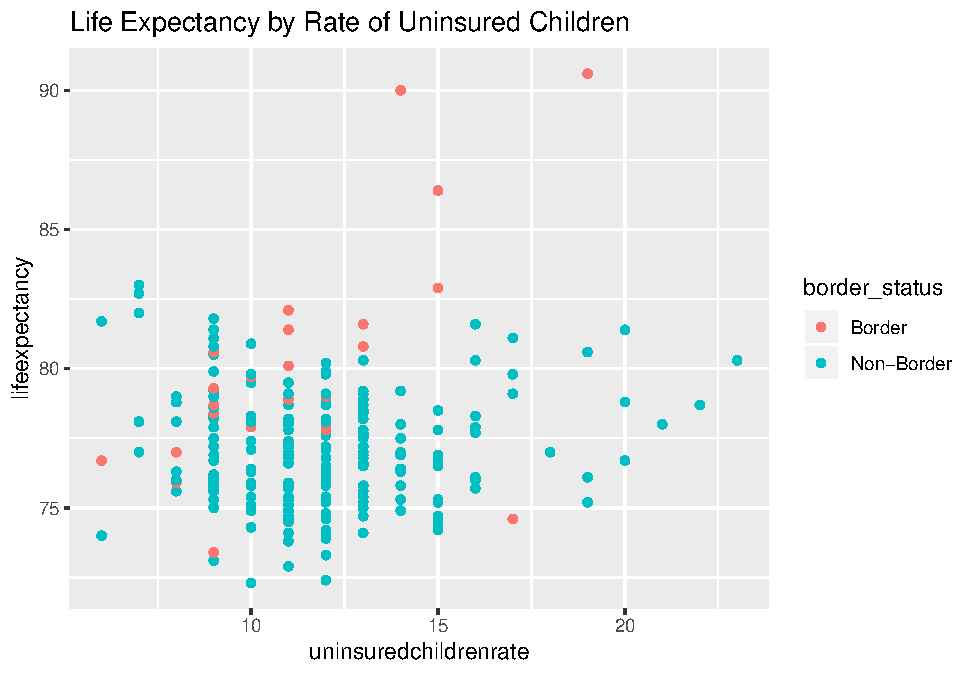
\includegraphics{2020-05-10-using-both-r-and-python-to-manipulate-data_files/figure-latex/unnamed-chunk-3-1.pdf}

As you can see, the data modifications made in Python played nicely with
the functions in R. This way, we can use Python code without losing the
benefits of ggplot, as we can use both simulatenously.

\end{document}
